\documentclass[11pt]{article}
% Basic Packages for Encoding (Input AND Output) and Langauge Support
\usepackage[utf8]{inputenc}
\usepackage[T1]{fontenc}
\usepackage[french]{babel}

% Change Layout with a User-Friendly Interface
\usepackage[margin=1in]{geometry}

% Include Pictures with a User-Friendly Interface
\usepackage{graphicx}
\usepackage{float}

% Extended Math Support from the Famous 'American Mathematical Society'
\usepackage{amsmath}
\usepackage{amsfonts}
\usepackage{amssymb}

% Just for Demonstration Purposes
\usepackage[math]{blindtext}

% For use on computer
\usepackage{hyperref}

% For table color
\usepackage{xcolor,colortbl}

% Tableau verticale
\usepackage{rotating}

% Figure dans figure
\usepackage{subfig}

% Multicolumn
\usepackage{multirow}

% Preuves
\usepackage{amsthm}

% Titre
\usepackage[affil-it]{authblk}
\title{\textbf{TP Caractérisation des condensateurs} \\ \textit{Géométrie et assemblage}}
\author{Camille Yerly, Romain Blondel}
\affil{2M8, Gymnase Auguste Piccard}

\begin{document}

\maketitle

\section{But}
Le but de ce travail pratique en deux parties est de vérifier, tout d'abord, les relations géométriques du condensateur puis, les lois d'assemblages de ceux-ci.
\section{Introduction}
Le condensateur est un dispositif permettant d'emmagasiner de l'énergie électrique. Il accumule l'énergie puis, la libère rapidement. Le condensateur est utilisé, par exemple, dans divers circuits électriques afin de stabiliser le courant, en se chargeant lors des pics de tensions et en se déchargeant lors des baisses de tentions.
\subsection{Expérience 1: Géométrie}
Dans cette expérience, nous avons utilisé un condensateur plan. La mesure de la capacité d'un condensateur repose sur la mesure de de sa décharge dans une résistance. Cette loi est donnée par: 
$$Q(t)_{decharge}=Q_0 \cdot e^{-\frac{t}{CR}}$$ 

\begin{proof}
Considérons une boucle d'un condensateur $C$ et d'une résistance $R$. Le condensateur possède alors une charge $q(t) = C U(t)$, tension qui est la même aux bornes de la résistance et produit un courant $I(t)$, et par la loi d'Ohm $U(t) = R I(t)$. Notons qu'ici $I(t) = - \frac{dq}{dt}$. On en déduit donc l'équation différentielle $q(t) = -RC \frac{dq}{dt} \Leftrightarrow q(t) = Q e^{-\frac{t}{RC}}$ comme pour $t=0$, $q(0) =Q$. On va utiliser l'équivalent avec la tension dans la suite du rapport $q(t) = Q e^{-\frac{t}{RC}} \Leftrightarrow C Q(t) = C Q_0 e^{-\frac{t}{RC}} \Leftrightarrow Q(t) = Q_0 e^{-\frac{t}{RC}} $ avec $Q(t)$ la tension qui sera par la suite également nommée $U$.
\end{proof}

Le produit $CR$ est la constante de temps du système. Cette expérience permet de vérifier la formule de base des condensateurs: 
$$C=\epsilon_0  \cdot \frac{S}{d}$$

\begin{proof}
Sans perte de temps en généralité, considérons une surface de Gauss enfermant la charge portée par l'une des plaques, ayant donc un flux $\Phi = ES$ ($E$ le champ électrique et $S$ la surface). Considérant le flux comme homogène et en négligeant les effets de bord, on obtient $ES = \frac{Q}{\epsilon_0}$, et par définition, la tension vaut $U = E d$ ($d$ la distance entre les plaques). On en conclut $C = \frac{Q}{U} = \frac{\epsilon_0 E S}{E d} = \epsilon_0 \frac{S}{d}$.
\end{proof}

Nous pouvons ajouter que la charge du condensateur décroît d'une façon exponentielle vers 0, partant de la charge Q (à $t=0$).  Après un laps de temps d'une constante de temps, ($t=CR$), la charge qui reste sur le condensateur est égale à $e^{-1} \approx 0.368 \approx 37\%$ de la charge contenue au départ. Après un temps égal à cinq ou dix fois la constante du temps, le condensateur peut être considéré comme déchargé.
\subsection{Expérience 2: Assemblage}
Les lois d'assemblage des condensateur en série et en parallèles sont similaires aux lois des assemblages de résistances déjà vus auparavant, mais elles sont en quelque sorte inversées. Les deux lois que cette expérience essai de vérifier sont pour les assemblage en parallèles : 
$$C_{tot}= \sum_i C_i$$

\begin{proof}
Sur un circuit en parallèle, on a $U_{tot} = U_i, \ \forall U_i$ et $Q_{tot} = \sum Q_i$. Comme $Q = CU$ et donc $Q_i = C_i U$, on obtient $Q_{tot} = \sum Q_i \Leftrightarrow C_{tot} U = \sum C_i U \Leftrightarrow C_{tot}= \sum C_i$.
\end{proof}

Et pour ceux en série : 
$$\frac{1}{C_{tot}}= \sum_i \frac{1}{C_i}$$

\begin{proof}
De même sur un circuit en série : $U_{tot} = \sum U_i$ et $Q_{tot} = Q_i, \ \forall Q_i$, et comme $Q = CU \Leftrightarrow U = \frac{Q}{C}$ (de même $U_i = \frac{Q}{C_i}$), on obtient $U_{tot} = \sum U_i \Leftrightarrow \frac{Q}{C_{tot}} = \sum \frac{Q}{C_i} \Leftrightarrow \frac{1}{C_{tot}}= \sum \frac{1}{C_i}$.
\end{proof}

\section{Principe de mesure et description}
\subsection{Matériel}

Afin de réaliser l'expérience 1 (géométrie), nous avons utilisé :
\begin{itemize}
\item Capacimètre
\item Condensateur plan
\item Interrupteur
\item Oscilloscope
\item Pied à coulisse
\item Générateur 
\item Divers câbles \\
\end{itemize}

Pour l'expérience 2 (assemblage) :
\begin{itemize}
\item Multimètre
\item Breadboard (plaque de montage de circuits)
\item Résistance (100 $[\Omega]$)
\item Différents condensateurs (10, 22 et 47 $[\mu F]$)
\item Générateur
\item Divers câbles
\end{itemize}

\subsection{Déroulement}
\subsubsection{Expérience 1 - Géométrie :} 
Nous avons réalisé cette expérience en deux parties.\\
Premièrement, il s'agissait de mesurer la capacité de du condensateur avec un capacimètre. 
\begin{enumerate}
\item Nous avons branché le condensateur plan au capacimètre à l'aide de deux câbles.
\item Nous avons mesuré la capacité du condensateur selon la distance entre les deux plaques, qui a été mesurée par le pied à coulisse. Nous avons pris les mesures tous les 1 $[mm]$ entre 1 $[mm]$ et 10 $[mm]$, tous les 5 $[mm]$ de 10 $[mm]$ à 40 $[mm]$ et tous les 20 $[mm]$ jusqu'à 80 $[mm]$. 
\end{enumerate}
Dans un deuxième temps, nous avons relevé la décharge du condensateur à l'aide d'un oscilloscope.
\begin{enumerate}
\item Nous avons branché le condensateur plan à l'oscilloscope, à l'interrupteur et au générateur grâce à divers câbles (voir figure \ref{fig:exp-schem1}) Dans ce montage, le condensateur se charge est se décharge grâce à l'interrupteur.
\item Nous avons réglé l'oscilloscope: l'échelle de la tension, le temps de mesure et le trigger pour déclencher la mesure. Nous avons également fixé une séquence unique de mesure avec une pente descendante.
\item Nous fait les mesures en déchargeant la courant, pour une distance de 1.5 $[cm]$, puis de 2 $[cm]$, entre les deux plaques.
\item nous avons relevé environ 15 mesures de la courbe affichée sur l'oscilloscope, à intervalles de tensions réguliers.
\end{enumerate} 
\subsubsection{Expérience 2 - Assemblage :}
Cette expérience s'est aussi faite en deux partie, semblablement à la première expérience; d'abord afin de mesurer les capacités avec le multimètre:
\begin{enumerate}
\item Nous avons mesurer la valeur des capacités de chaque condensateur à l'aide du multimètre.
\item Nous avons monté trois assemblages de condensateurs (série, parallèle et mixte) comme sur la figure \ref{fig:cap-schem2}.
\item Nous avons branché le multimètre à chaque extrémité des circuits et avons ainsi mesuré la capacité de chaque assemblage.
\end{enumerate}
Puis pour relever la décharge sur l'oscilloscope:
\begin{enumerate}
\item Nous avons ajouté une résistance de 100 $[\Omega]$ et avons branché l'oscilloscope, ainsi que le générateur, sur l'assemblage en série selon la figure \ref{sfig:osc-schem2_ser}.
\item Nous avons réglé les échelles de tensions et de temps de l'oscilloscope afin d'avoir une mesure centrée. Nous avons aussi réglé le trigger et la séquence unique de mesure, semblablement à l'expérience 1.
\item Nous avons effectué les mesures en déchargeant le circuit au moyen des câbles.
\item Nous avons relevé environ 10 mesures de la tension selon le temps sur l'oscilloscope.
\item Nous avons réitéré cette partie de l'expérience pour l'assemblage en parallèle. Le montage a été fait identiquement à la figure \ref{sfig:osc-schem2_par}.
\end{enumerate}

\subsection{Schémas}

Ci-dessous les schémas de nos montages, avec les différentes valeurs sur les condensateurs (en gris) et résistances (en blanc) ; la couleur des câbles est purement pratique, sauf celui noir et gris qui correspond à celui de l'oscilloscope.

\subsubsection*{Géométrie}

Le système permet de régler l'écart entre les plaque, mais la réglette est pas très précise donc on a ajusté $d$ avec un pied à coulisse.

\begin{figure}[H]
\centering
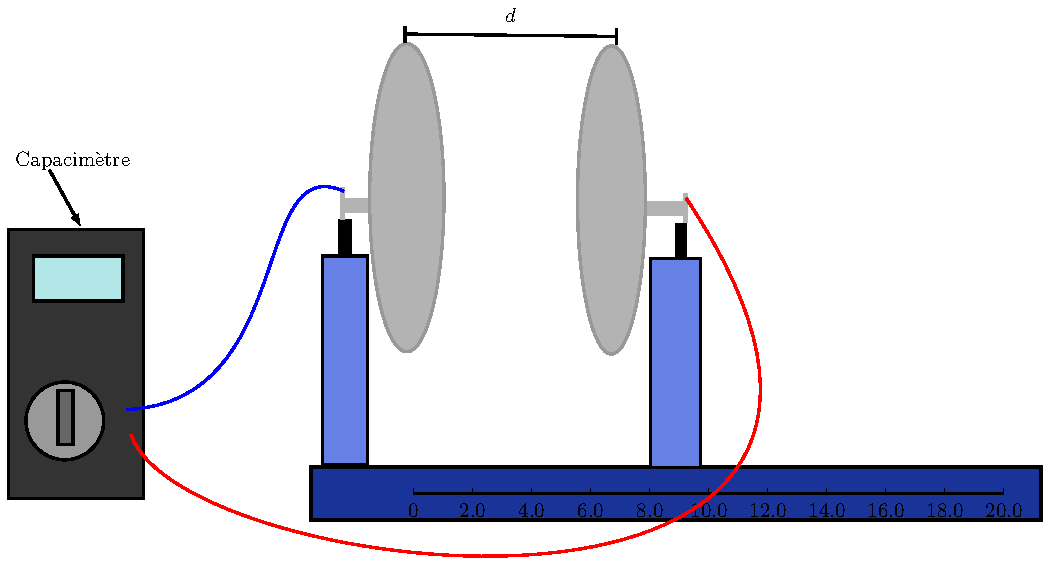
\includegraphics[scale=0.5]{Images/mesure1_capa.pdf}
\caption{Montage autour du condensateur plan (mesure au capacimètre)}
\label{fig:cap-schem1}
\end{figure}

Pour faciliter la charge/décharge du condensateur, on a utilisé un interrupteur dans le montage.

\begin{figure}[H]
\centering
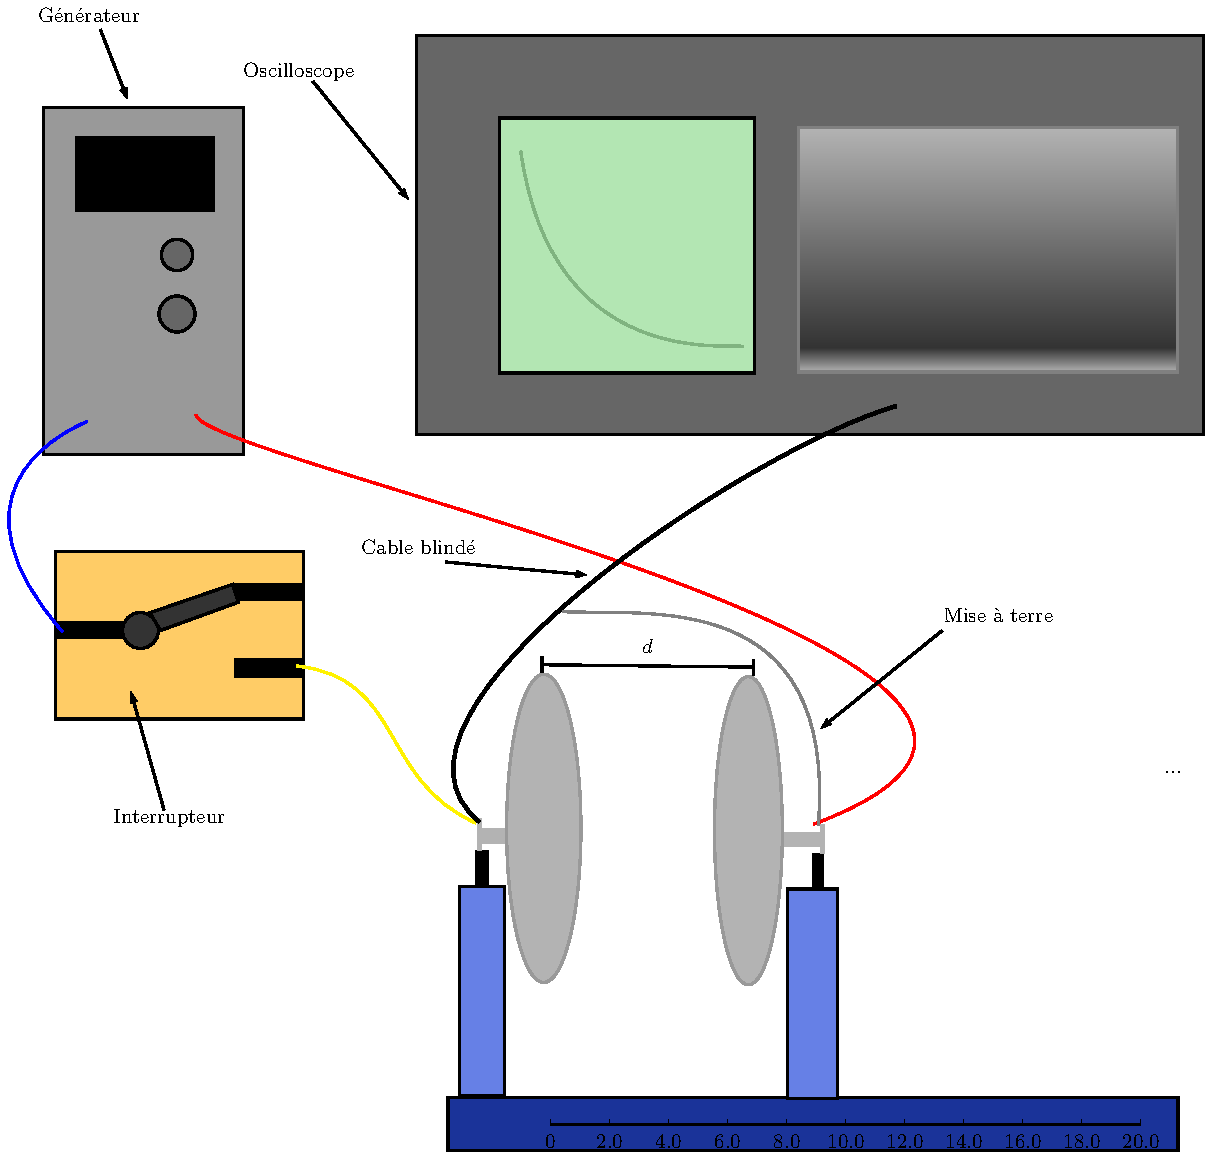
\includegraphics[scale=0.5]{Images/mesure1_osc.pdf}
\caption{Montage autour du condensateur plan (mesure à l'oscilloscope, activer l'interrupteur pour lancer la mesure)}
\label{fig:exp-schem1}
\end{figure}

\subsubsection*{Assemblage}

La figure \ref{fig:cap-schem2} résume nos circuits d’assemblage complets ; pour les mesures entre uniquement deux condensateurs, c'est le même principe, et pour un unique on branche juste aux bornes.

\begin{figure}[H]
\centering
\subfloat[En série\label{sfig:cap-schem2_ser}]{%
   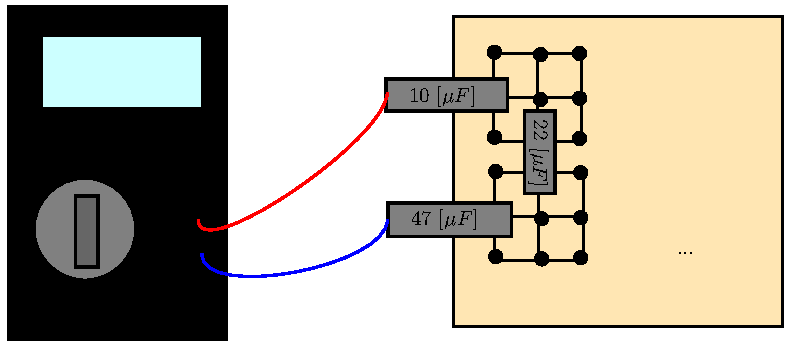
\includegraphics[width=0.49\linewidth]{Images/mesure2_ser_capa.pdf}}\hfill
\subfloat[En parallèle\label{sfig:cap-schem2_par}]{%
   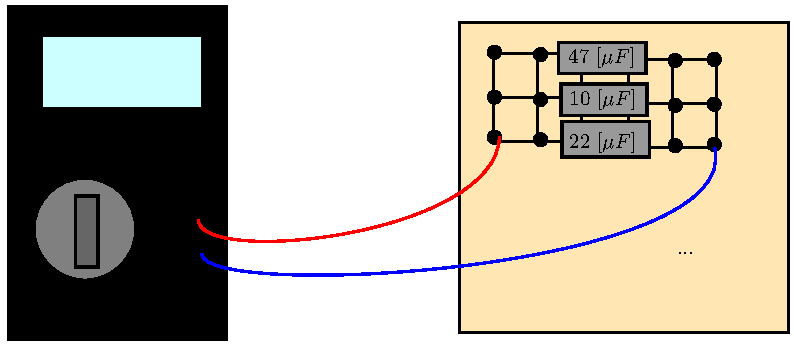
\includegraphics[width=0.49\linewidth]{Images/mesure2_par_capa.pdf}}\hfill
\subfloat[Mixte\label{sfig:cap-schem2_mixte}]{%
   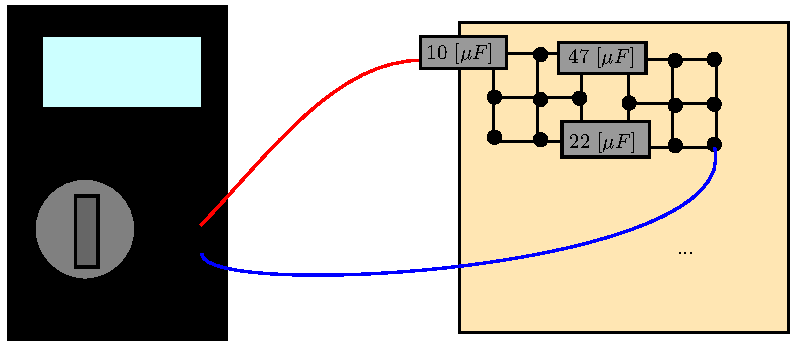
\includegraphics[width=0.49\linewidth]{Images/mesure2_mixte_capa.pdf}}\hfill
\caption{Montage d'assemblage (mesure au capacimètre)}
\label{fig:cap-schem2}
\end{figure}

L'ajout d'un résistance est importante afin de mesurer la décroissance exponentielle.

\begin{figure}[H]
\centering
\subfloat[En série\label{sfig:osc-schem2_ser}]{%
   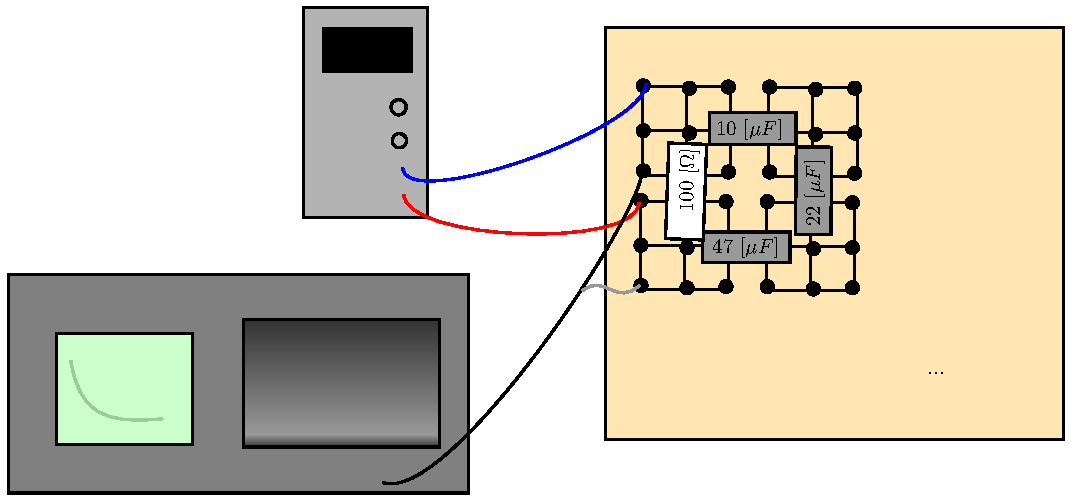
\includegraphics[width=0.5\linewidth]{Images/mesure2_ser_osc.pdf}}\hfill  
\subfloat[En parallèle\label{sfig:osc-schem2_par}]{%
   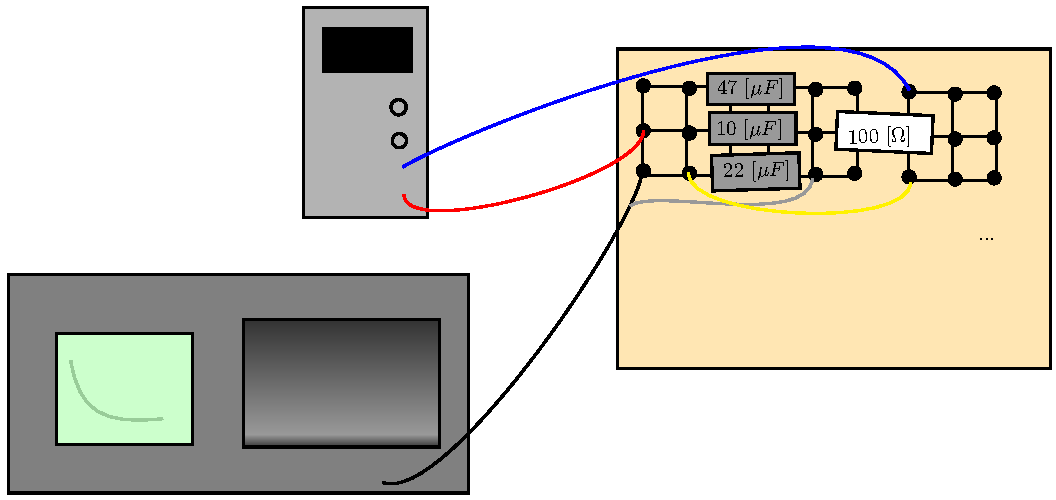
\includegraphics[width=0.5\linewidth]{Images/mesure2_par_osc.pdf}}\hfill
\caption{Montage d'assemblage (mesure à l'oscilloscope, débrancher le câble bleu ou rouge pour lancer la mesure)}
\label{fig:exp-schem2}
\end{figure}

\section{Résultats et calculs}

Les résultats et calculs sont consignés en deux parties. Tout d'abord ceux traitant de la géométrie des condensateurs, et ensuite ceux pour l'assemblage.

\subsection*{Géométrie}

La table \ref{tab:cap_geo} résume nos mesures, selon la distance $d$ entre les plaques du condensateur, de la capacité $C_{mes}$. Les mesures doivent être corrigées à cause d'une capacité parasite de $0.041 \ [nF]$, d'où $C_{corr} = C_{mes} - (0.041 \ [nF])$. Il est aussi important de connaître la capacité théorique via la formule des condensateurs plans $C_{th} = \epsilon_0 \frac{S}{d} $ où $\epsilon_0 \approx 8.854187 \cdot 10^{-12} \ [F/m]$ est la constante de permittivité du vide, $S = \pi \cdot 0.099^2 \approx 0.03079 \ [m^2]$ la surface du condensateur (qui a donc un rayon de $9.9 \ [cm]$) et $d$ la distance entre les plaques. Ensuite sont consignés pour une utilisation ultérieur l'inverse de la distance, et finalement l'erreur relative $\vert \frac{C_{corr} - C_{th}}{C_{th}} \vert$ entre la capacité corrigée et celle théorique.

\begin{table}[H]
\resizebox{\columnwidth}{!}{
\begin{tabular}{|>{\columncolor{darkgray}}c|c|>{\columncolor{gray}}c|c|>{\columncolor{gray}}c|c|>{\columncolor{gray}}c|c|>{\columncolor{gray}}c|c|>{\columncolor{gray}}c|c|>{\columncolor{gray}}c|c|>{\columncolor{gray}}c|c|>{\columncolor{gray}}c|>{\columncolor{gray}}c|c|}
\hline 
$d \ [mm]$ & 1 & 2 & 3 & 4 & 5 & 6 & 7 & 8 & 9 & 10 & 15 & 20 & 25 & 30 & 35 & 40 & 60 & 80 \\ 
\hline 
$C_{mes} \ [nF]$ & 0.34 & 0.187 & 0.15 & 0.105 & 0.092 & 0.083 & 0.074 & 0.074 & 0.085 & 0.069 & 0.07 & 0.052 & 0.064 & 0.055 & 0.048 & 0.045 & 0.048 & 0.049 \\ 
\hline 
\hline
$C_{corr} \ [nF]$ & 0.299 & 0.146 & 0.109 & 0.064 & 0.051 & 0.042 & 0.033 & 0.033 & 0.044 & 0.028 & 0.029 & 0.011 & 0.023 & 0.014 & 0.007 & 0.004 & 0.007 & 0.008 \\
\hline
$C_{th} \ [nF]$  & 0.273 & 0.136 & 0.091 & 0.068 & 0.055 & 0.045 & 0.039 & 0.034 & 0.03 & 0.027 & 0.018 & 0.014 & 0.011 & 0.009 & 0.008 & 0.007 & 0.005 & 0.003 \\
\hline
\hline
$1/d \ [m^{-1}]$ & 1000 & 500 & 333.33 & 250 & 200 & 166.67 & 142.86 & 125 & 111.11 & 100 & 66.67 & 50 & 40 & 33.33 & 28.57 & 25 & 16.67 & 12.5 \\ 
\hline 
\hline
Erreur $[\%]$ & 9.67 & 7.11 & 19.94 & 6.10 & 6.47 & 7.57 & 15.28 & 3.16 & 45.25 & 2.70 & 59.56 & 19.30 & 110.91 & 54.06 & 10.13 & 41.31 & 54.06 & 134.75 \\ 
\hline 
\end{tabular}}
\caption{Mesures et calculs sur le montage \ref{fig:cap-schem1}}
\label{tab:cap_geo}
\end{table}

Le graphique suivant montre la relation de proportionalité entre la capacité et l'inverse de la distance de la formule $C_{th} = \epsilon_0 \frac{S}{d} $, ainsi que l'importance de la correction.

\begin{figure}[H]
\centering
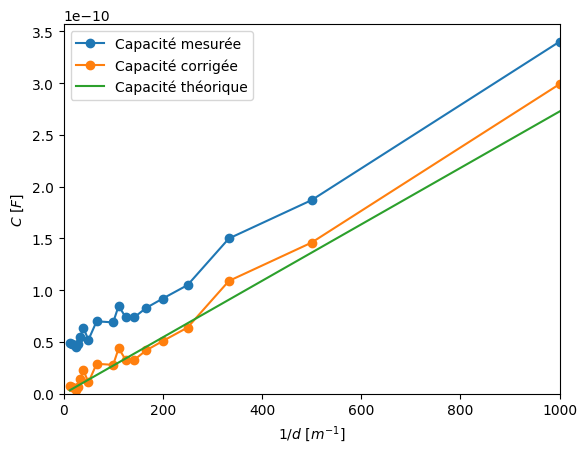
\includegraphics[scale=0.7]{Images/comp-cap.png}
\caption{Capacité mesurée et théorique}
\label{fig:comp-cap}
\end{figure}

Afin de mieux visualiser l'erreur, on en a établit un diagramme (moyenne à $33.74 \ [\%]$).
\begin{figure}[H]
\centering
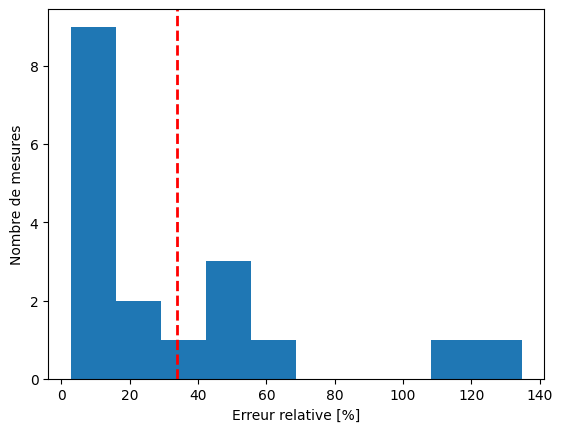
\includegraphics[scale=0.5]{Images/histo-err.png}
\caption{Histogramme d'erreur (moyenne en rouge)}
\label{fig:histo-err}
\end{figure}

Deuxièmement sont consignées nos mesures de la tension lors de la décharge à l'oscilloscope, afin de calculer la capacité via la propriété de décroissance exponentielle $Q(t) = Q_0 \cdot e^{- \frac{1}{RC} \cdot t}$, avec $Q$ la tension en volts, $R$ la résistance du circuit, $C$ la capacité, $t$ le temps et $e$ le nombre d’Euler.

\begin{table}[H]
\subfloat[{$d=1.5 \ [cm]$}\label{stab:dec15}]{%
\resizebox{\columnwidth}{!}{\begin{tabular}{|>{\columncolor{darkgray}}c|c|>{\columncolor{gray}}c|c|>{\columncolor{gray}}c|c|>{\columncolor{gray}}c|c|>{\columncolor{gray}}c|c|>{\columncolor{gray}}c|c|>{\columncolor{gray}}c|c|>{\columncolor{gray}}c|c|>{\columncolor{gray}}c|}
\hline 
$t \ [\mu s]$ & 0 & 20 & 40 & 60 & 80 & 100 & 120 & 140 & 160 & 180 & 200 & 250 & 300 & 400 & 500 & 600 \\ 
\hline 
$Q(t) \ [V]$ & 8.4 & 7.52 & 6.8 & 6.08 & 5.52 & 4.96 & 4.48 & 4 & 3.6 & 3.28 & 2.96 & 2.24 & 1.76 & 1.04 & 0.48 & 0.4 \\ 
\hline 
\end{tabular}}}\hfill
\subfloat[{$d=2 \ [mm]$}\label{stab:dec2}]{%
\resizebox{\columnwidth}{!}{\begin{tabular}{|>{\columncolor{darkgray}}c|c|>{\columncolor{gray}}c|c|>{\columncolor{gray}}c|c|>{\columncolor{gray}}c|c|>{\columncolor{gray}}c|c|>{\columncolor{gray}}c|c|>{\columncolor{gray}}c|c|}
\hline 
$t \ [\mu s]$ & 0 & 50 & 100 & 150 & 200 & 250 & 300 & 350 & 400 & 450 & 500 & 550 & 600 \\ 
\hline 
$Q(t) \ [V]$ & 8.56 & 6.96 & 6.08 & 5.04 & 4.32 & 3.5 & 3.04 & 2.5 & 2.08 & 1.7 & 1.52 & 1.2 & 1.12 \\ 
\hline 
\end{tabular}}}\hfill
\caption{Mesure de la tension en fonction du temps}
\label{tab:mesqt_geo}
\end{table}

De là, on calcule la courbe de tendance afin d'ajuster nos données à une fonction du type $f(t) = A \cdot e^{-B \cdot t}$, en l’occurrence via la méthode des moindres carrés.

\begin{figure}[H]
\centering
\subfloat[{$d=1.5 \  [cm]$}\label{sfig:dec15}]{%
   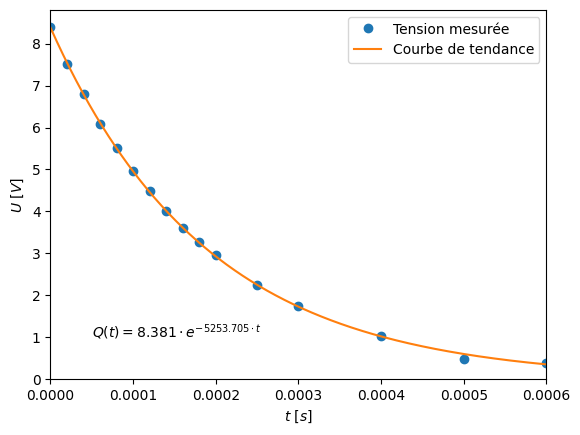
\includegraphics[width=0.49\linewidth]{Images/dec1.png}}\hfill 
\subfloat[{$d=2 \  [mm]$}\label{sfig:dec2}]{%
   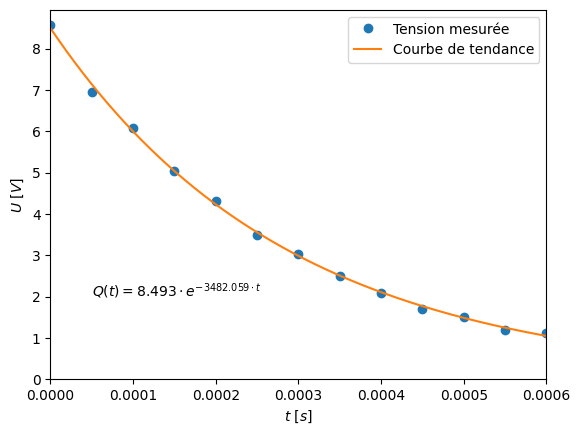
\includegraphics[width=0.49\linewidth]{Images/dec2.png}}\hfill 
\caption{Décroissances exponentielles}
\label{fig:decgeo}
\end{figure}

Pour la distance $d=1.5 \  [cm]$ (Figure \ref{sfig:dec15}), on obtient un $Q_0 \approx 8.381 \ [V]$, ce qui par rapport à notre mesure à $t=0$ fait $0.23 \ [\%]$ d'erreur. Pour ce qui est de la capacité, on estime la résistance comme celle interne du circuit à $R=2 \ [M \Omega]$, et donc $\frac{1}{RC} \approx 5253.705 \Leftrightarrow C \approx \frac{1}{R \cdot 5253.705} \approx 0.0952 \ [nF]$, ce qui fait une différence de $35.96 \ [\%]$ par rapport à l'autre mesure et donc $228.18 \ [\%]$ une fois corrigée.\\
Pour celle $d=2 \  [mm]$ (Figure \ref{sfig:dec2}), $Q_0 \approx 8.493 \ [V]$ et donc une erreur de $0.79 \ [\%]$ par rapport à la mesure, et on obtient également $\frac{1}{RC} \approx 3482.059 \Leftrightarrow C \approx 0.144 \ [nF]$, donc $23.21 \ [\%]$ d'erreur par rapport à la mesure, mais $1.65 \ [\%]$ par rapport à la mesure corrigée.

\subsection*{Assemblage}

Les mesures sur les assemblages de condensateurs sont consignées ci-dessous. On garde les nominations tel quel, mais la capacité des condensateur n'est pas la même : celui "10" a une capacité de $9.31  \ [\mu F]$, "22" a $23.98 \ [\mu F]$ et "47" $55.7 \ [\mu F]$ (ces capacités corrigées ont été mesurée avant de faire les montages). La capacité théorique est donc calculée à partir des ces mesures, et via les règles d'assemblage : $\frac{1}{C_{ser}} = \sum \frac{1}{C_{i}}$ et $C_{par} = \sum C_i$. La table \ref{tab:cap_cirass} résume donc les mesures des circuits en figure \ref{fig:cap-schem2}, ainsi que les sous assemblages. Donc, pour le circuit \ref{sfig:cap-schem2_ser}, la capacité vaut $\frac{1}{C_{tot}} = \frac{1}{C_{10}}+\frac{1}{C_{22}}+\frac{1}{C_{47}} \Leftrightarrow C_{tot} = (\frac{1}{C_{10}}+\frac{1}{C_{22}}+\frac{1}{C_{47}})^{-1}$ ; pour \ref{sfig:cap-schem2_par}, $C_{tot}= C_{10} + C_{22} + C_{47}$ ; finalement, pour \ref{sfig:cap-schem2_mixte}, on fait l'assemblage "22-47" en parallèle puis avec "10" en série $C_{tot} = (\frac{1}{C_{22}}+\frac{1}{C_{47}})^{-1} + C_{10}$.

\begin{table}[H]
\centering
\begin{tabular}{|>{\columncolor{darkgray}}c||c|>{\columncolor{gray}}c|c|>{\columncolor{gray}}c||c|>{\columncolor{gray}}c|c|>{\columncolor{gray}}c||c|}
\hline 
\rowcolor{darkgray} \cellcolor{black} & \multicolumn{4}{|c||}{En série} & \multicolumn{4}{|c||}{En parallèle} & Mixte \\ 
\hline 
Assemblage & $\circ$ & 10-22 & 10-47 & 22-47 & $\circ$ & 10-22 & 10-47 & 22-47 & $\circ$ \\ 
\hline 
$C_{mes} \ [\mu F]$ & 5.91 & 6.67 & 7.92 & 16.61 & 90.2 & 33.58 & 65.4 & 80.2 & 26.21 \\ 
\hline 
$C_{th} \ [\mu F]$ & 5.99 & 6.71 & 7.98 & 16.76 & 88.99 & 33.29 & 65.01 & 79.68 & 26.07 \\ 
\hline 
Erreur $[\%]$ & 1.28 & 0.55 & 0.72 & 0.922 & 1.341 & 0.86 & 0.60 & 0.648 & 0.522 \\ 
\hline 
\end{tabular} 
\caption{Mesure des capacités des circuits ($\circ$ : circuit complet)}
\label{tab:cap_cirass}
\end{table}

Ensuite, les mesures on été à nouveau faite selon la méthode de la décroissance exponentielle sur le circuit en parallèle et celui en série.

\begin{table}[H]
\subfloat[{En parallèle}\label{stab:decpar}]{%
\resizebox{\columnwidth}{!}{\begin{tabular}{|>{\columncolor{darkgray}}c|c|>{\columncolor{gray}}c|c|>{\columncolor{gray}}c|c|>{\columncolor{gray}}c|c|>{\columncolor{gray}}c|c|>{\columncolor{gray}}c|c|}
\hline 
$t \ [m s]$ & 0 & 2.5 & 5 & 7.5 & 10 & 12.5 & 15 & 17.5 & 20 & 22.5 & 25 \\ 
\hline 
$Q(t) \ [V]$ & 8.32 & 6.08 & 4.64 & 3.5 & 2.72 & 2.1 & 1.6 & 1.2 & 1.04 & 0.75 & 0.56 \\ 
\hline 
\end{tabular}}}\hfill
\subfloat[{En série}\label{stab:decser}]{%
\resizebox{\columnwidth}{!}{\begin{tabular}{|>{\columncolor{darkgray}}c|c|>{\columncolor{gray}}c|c|>{\columncolor{gray}}c|c|>{\columncolor{gray}}c|c|>{\columncolor{gray}}c|c|>{\columncolor{gray}}c|c|>{\columncolor{gray}}c|}
\hline 
$t \ [m s]$ & 0.1 & 0.2 & 0.3 & 0.4 & 0.5 & 0.6 & 0.7 & 0.8 & 0.9 & 1 & 1.1 & 1.2 \\ 
\hline 
$Q(t) \ [V]$ & 9.12 & 7.68 & 6.4 & 5.36 & 4.56 & 3.84 & 3.28 & 2.8 & 2.32 & 2 & 1.76 & 1.44 \\ 
\hline 
\end{tabular}}}\hfill
\caption{Mesure de la tension en fonction du temps}
\label{tab:mesqt_ass}
\end{table}

\begin{figure}[H]
\centering
\subfloat[{En parallèle}\label{sfig:decpar}]{%
   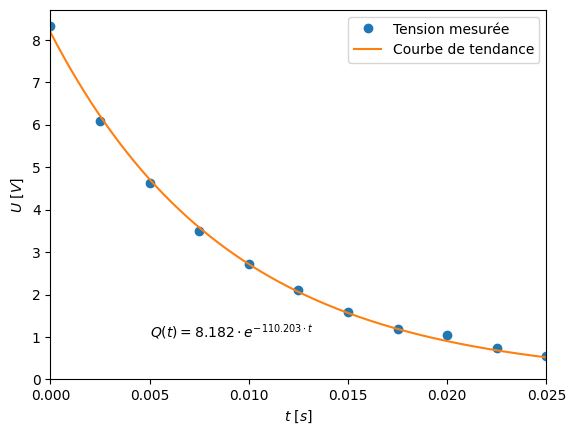
\includegraphics[width=0.49\linewidth]{Images/dec3.png}}\hfill 
\subfloat[{En série}\label{sfig:decser}]{%
   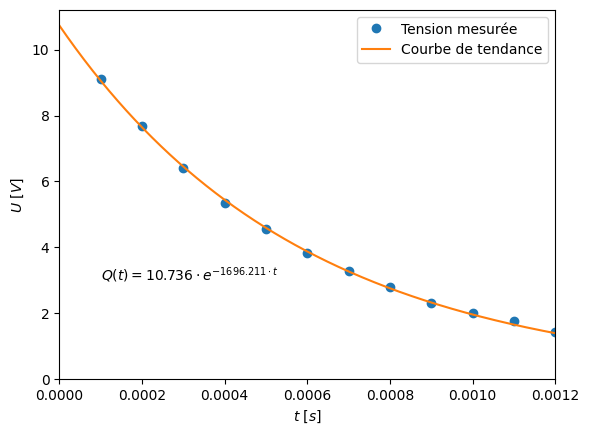
\includegraphics[width=0.49\linewidth]{Images/dec4.png}}\hfill 
\caption{Décroissance exponentielle des circuits}
\label{fig:decass}
\end{figure}

Ce qui nous donne en suivant la même procédure que précédemment pour le circuit en parallèle (figure \ref{sfig:decpar}) une tension $Q_0 \approx 8.182 \ [V]$ qui nous donne une erreur par rapport à la mesure en $t=0$ de $1.66 \ [\%]$. Sachant que la résistance sur le circuit est celle que l'on à ajouté, soit de $100 \ [\Omega]$, l'exposant $110.203$ nous permet de calculer $C = 90.74 \ [\mu F]$. Cela nous donne $0.60 \ [\%]$ d'erreur avec la mesure et $1.93 \ [\%]$ avec le calcul théorique.\\
Pour le circuit en série (figure \ref{sfig:decser}), on ne peut pas comparer $Q_0$, n'ayant pas de mesure à $t_0$. L'exposant $1696.211$ nous permet de calculer $C = 5.90 \ [\mu F]$, donc une erreur vis à vis de la mesure de $0.25 \ [\%]$ et $1.53 \ [\%]$ par rapport au calcul théorique.

\section{Discussion des résultats}

Les résultats semblent globalement assez bon. On observe bien sur la figure \ref{fig:comp-cap} la relation entre l'inverse de la distance et la capacité, selon la formule $C = \epsilon_0 \frac{S}{d}$ pour les condensateurs plan. Néanmoins, on observe également des erreurs assez grosses (figure \ref{fig:histo-err}). On observe en effet une seule mesure sous $5 \ [\%]$ d'erreur, malgré tout une majorité de mesure sous les $20 \ [\%]$, mais néanmoins un nombre significatif au dessus ce qui mène à une moyenne de $33.74 \ [\%]$, ce qui avec les deux mesures à plus de $100 \ [\%]$, pourrait faire douter de la méthode. Il faut pourtant nuancer ce propos car l'on était aux limites de la capacité de mesure du capacimètre, comme en témoigne le courant parasite, ainsi qu'avec des valeurs tellement faible que les moindre problèmes ont un gros impacte. En effet, pour les deux mesures avec plus de $100 \ [\%]$ d'erreur, la capacité parasite représente $83.67 \ [\%]$ et $64.06 \ [\%]$ de la mesure initiale, ce qui montre une relative imprécision de l'appareil vers ces valeurs. \\ \\
Des constats similaires peuvent être établi pour la décroissance exponentielle, où les faible valeurs montre une erreur énorme sur la mesure la plus petite - $d = 1.5 \ [cm]$ ($35 \ [\%]$ par rapport à la mesure - qui est elle même à $59.56 \ [\%]$ - et $228.18 \ [\%]$ avec la théorie), mais plusieurs raisons peuvent être envisagée, tel que le montage (mouvement de l'interrupteur, ...) ou plus probablement la résistance considérée, qui est une estimation et non de notre propre mesure. Quand la capacité est plus grande, on observe néanmoins une grande précision de la décroissance exponentielle, car pour $d= 2 \ [mm]$, l'erreur vis à vis de la mesure corrigée est à $1.65 \ [\%]$. \\ \\
Pour l'assemblage, l'erreur est presque nulle, moins de $1 \ [\%]$ entre deux condensateur, petite erreur qui se répercute quand on les assembles à plusieurs, mais reste inférieur à $2 \ [\%]$. Le point le plus étonnant est la différence entre la capacité nominale et celle réel. À l'aide de la décroissance exponentielle, on observe que les deux mesures se valent (moins de $1 \ [\%]$ entre les deux), mais toujours un peu moins de $2 \ [\%]$ vis à vis de la théorie, ce qui laisse penser qu'il nous manque des paramètres, probablement la résistance interne du circuit, comme la mesure de la capacité est inférieur à celle calculée. \\ \\
On peut donc noter des théories très puissantes, mais une mesure assez complexe du à des valeurs en générale très petites. Le capacimètre permet une mesure bien plus simple, mais la mesure de la décroissance et son approximation est aussi très intéressant pour montrer la validité d'autres résultats et pouvoir envisager différents moyens pour vérifier la pertinence des valeurs.

\section{Conclusion}

En conclusion, on peut noter d'assez bon résultats. De part leur taille, ils sont très sensibles aux paramètres extérieurs, donc il serait intéressant de les quantifier afin de pouvoir les éliminer. Il est également envisageable d'augmenter la tension, ou tout autre paramètre, afin de les rendre négligeables. De plus, il serait intéressant de mener des mesures avec des appareils plus précis, comme le capacimètre ou une méthode de calibrage de la distance $d$ suffisamment bon directement dans le dispositif plutôt que d'utiliser un outil extérieur, en l’occurrence le pied à coulisse. Malgré tout, cela confirme la théorie et on voit sur l'assemblage qu'avec des valeurs plus grande les mesures sont très précises.

\end{document}